\section{Experiments}
\label{sec:experiments}

We answer four questions. \textbf{Q1} Does simulated data transfer to objects with no real data, and which renderer is needed? \textbf{Q2} How does the benefit scale with the real budget $\Kreal$ for each renderer family? \textbf{Q3} How much does renderer leakage inflate the measured benefit? \textbf{Q4} Can renderer fidelity be measured without training the downstream model, and which appearance factors limit it?

All numbers are real-frame errors of the downstream model; depth MSE in $\mathrm{mm}^2$, contact MAE in mm, rotation in degrees. Depth metrics use the checkpoint with the lowest validation depth MSE and pose metrics the checkpoint with the lowest validation angular error, both selected on the seen-object validation split only.

\subsection{Q1: Transfer to Unseen Objects}
\label{sec:loo}

\begin{table}[t]
\centering
\tableformat
\caption{\textbf{Leave-object-out.} Errors on $1{,}244$ real frames of three objects with no real training data. Rows add simulated contacts of all 12 meshes to the real frames of the nine other objects, unless noted. Leaky: renderer trained on real frames of the held-out objects. Bold: best leakage-free.}
\label{tab:loo}
\begin{tabularx}{\columnwidth}{Xrrrrr}
\toprule
Training data & \metrichead{Depth}{MSE} & \metrichead{Contact}{MAE} & \shortstack[c]{\strut Contact\\\strut IoU\,$\uparrow$} & \metrichead{Rot.}{(deg)} & \metrichead{Trans.}{$L_1$} \\
\midrule
Real only (9 objects) & 0.0659 & 0.347 & 0.587 & 48.3 & 0.088 \\
+ Blender & 0.0675 & 0.352 & 0.587 & 7.8 & \textbf{0.035} \\
+ Blender, bg-norm. & 0.0662 & 0.348 & 0.591 & \textbf{5.6} & 0.036 \\
+ GAN-LOO & \textbf{0.0612} & \textbf{0.333} & \textbf{0.617} & 7.6 & 0.039 \\
\quad w/o held-out meshes & 0.0622 & 0.337 & 0.609 & 55.3 & 0.067 \\
+ diff-GAN-LOO & 0.0627 & 0.346 & 0.607 & 6.3 & 0.040 \\
\midrule
\textit{+ GAN-full (leaky)} & \textit{0.0455} & \textit{0.281} & \textit{0.677} & \textit{6.7} & \textit{0.037} \\
\midrule
\multicolumn{6}{@{}l}{\textit{Reference: same models on the nine seen objects}} \\
Real only & 0.0115 & 0.109 & 0.874 & 3.8 & 0.021 \\
+ GAN-LOO & 0.0094 & 0.106 & 0.884 & 5.8 & 0.029 \\
\bottomrule
\end{tabularx}
\end{table}

\begin{figure}[t]
    \centering
    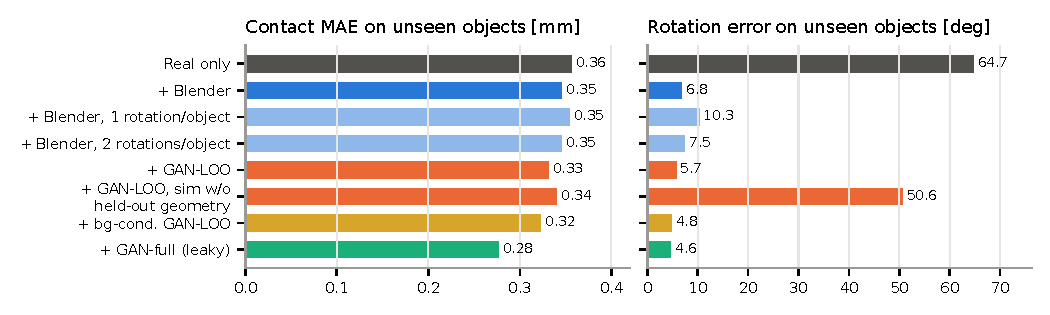
\includegraphics[width=\columnwidth]{figures/fig_loo.pdf}
    \caption{\textbf{Unseen objects (Table~\ref{tab:loo}).} Simulated contacts of a new mesh make its pose estimable with either renderer; removing the mesh from simulation (geometry control) removes the gain. Contact depth error barely moves without leakage.}
    \label{fig:loo}
\end{figure}

Table~\ref{tab:loo} and Fig.~\ref{fig:loo} give the leave-object-out results. Without any data of the three objects, the pose head fails: $48.3^\circ$ mean rotation error, which is chance level for the two-fold symmetric patterns. Adding simulated contacts of the three meshes reduces this to $7.8^\circ$ with the physically calibrated renderer---calibrated from a single no-contact frame and never shown a real contact of any object---and to $5.6^\circ$ when per-session illumination is normalized (Sec.~\ref{sec:negative}). The learned renderer reaches $7.6^\circ$ (strict) and $6.7^\circ$ (leaky); the leaky variant buys little for pose. The geometry control isolates the cause: the same GAN-LOO renderer with the three meshes removed from simulation gives $55.3^\circ$, i.e.\ no transfer. Pose transfer is driven by geometric coverage of the new object in simulation, and any renderer that preserves the contact silhouette suffices.

Dense depth behaves differently. Contact MAE on the unseen objects is $0.35\,$mm for real-only training---three times the $0.11\,$mm on seen objects---and no leakage-free renderer reduces it by more than $4\%$ (GAN-LOO: $0.333$, IoU $0.59\!\to\!0.62$). The geometry control gives almost the same depth ($0.337$), so the small gain is a regularization effect of additional synthetic frames rather than object coverage. Only the leaky renderer, which has seen real contacts of these objects, reduces contact MAE substantially ($0.281$, $-19\%$). Cross-object depth generalization is thus limited by contact appearance, and the leaky number is not achievable without real touches of the object. Peak-depth error is small for every row ($0.05$--$0.08\,$mm at $\approx1\,$mm indentation): the models estimate \emph{how deep} correctly and err in \emph{where} the contact region lies (IoU $\approx0.6$).

\subsection{Q2: Real-Data Budget}
\label{sec:kshot}

\begin{table}[t]
\centering
\tableformat
\caption{\textbf{$\Kreal$-shot with a shared real budget.} Every object contributes $\Kreal$ real frames; GAN-$\Kreal$ is trained on the same frames. Real validation split ($472$ frames). Leaky rows use the renderer trained on all real pairs.}
\label{tab:kshot}
\begin{tabularx}{\columnwidth}{lXrrrr}
\toprule
$\Kreal$ & Training data & \metrichead{Depth}{MSE} & \metrichead{Contact}{MAE} & \shortstack[c]{\strut IoU\\\strut $\uparrow$} & \metrichead{Rot.}{(deg)} \\
\midrule
0 & Blender only & 0.0786 & 0.406 & 0.574 & 9.0 \\
  & \textit{GAN-full only (leaky)} & \textit{0.0464} & \textit{0.275} & \textit{0.705} & \textit{8.0} \\
\midrule
10 & Real only & 0.0639 & \textbf{0.329} & \textbf{0.627} & 10.1 \\
   & + Blender & 0.0633 & 0.366 & 0.600 & \textbf{6.3} \\
   & + GAN-10 & \textbf{0.0620} & 0.348 & 0.596 & 6.7 \\
   & \textit{+ GAN-full (leaky)} & \textit{0.0484} & \textit{0.281} & \textit{0.693} & \textit{6.1} \\
\midrule
25 & Real only & 0.0558 & \textbf{0.303} & \textbf{0.666} & \textbf{5.5} \\
   & + Blender & 0.0569 & 0.347 & 0.659 & 5.6 \\
   & + GAN-25 & \textbf{0.0539} & 0.318 & 0.619 & 5.9 \\
   & \textit{+ GAN-full (leaky)} & \textit{0.0423} & \textit{0.254} & \textit{0.725} & \textit{5.9} \\
\midrule
100 & Real only & 0.0367 & 0.238 & 0.746 & \textbf{3.9} \\
    & + Blender & 0.0341 & 0.220 & 0.760 & 5.3 \\
    & + GAN-100 & \textbf{0.0299} & \textbf{0.202} & \textbf{0.780} & 5.5 \\
    & \textit{+ GAN-full (leaky)} & \textit{0.0273} & \textit{0.191} & \textit{0.791} & \textit{5.4} \\
\bottomrule
\end{tabularx}
\end{table}

\begin{figure*}[t]
    \centering
    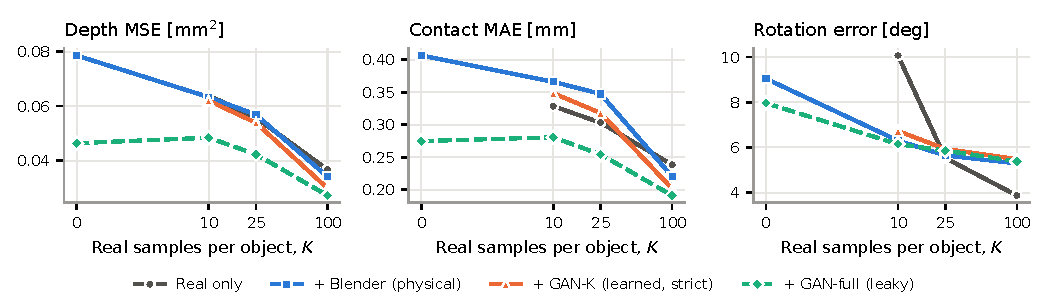
\includegraphics[width=0.95\textwidth]{figures/fig_kshot.pdf}
    \caption{\textbf{Real-data budget (Table~\ref{tab:kshot}).} Real validation error versus real frames per object. The strict learned renderer (GAN-$\Kreal$, trained on the same $\Kreal$ frames) separates from real-only training only at $\Kreal=100$; the physical renderer never improves depth. The leaky renderer (dashed) appears to help at every $\Kreal$. Rotation benefits from simulation only at $\Kreal\le10$.}
    \label{fig:kshot}
\end{figure*}

Table~\ref{tab:kshot} and Fig.~\ref{fig:kshot} vary the real budget. Three regimes appear.

\noindent\textbf{Zero-shot ($\Kreal=0$).} Simulation alone transfers poorly for depth: contact MAE $0.41\,$mm with the physical renderer, versus $0.11\,$mm reachable with the full real set. The leaky learned renderer halves this ($0.275$), but it has seen $4{,}197$ real pairs, so it is not a zero-shot result.

\noindent\textbf{Few-shot ($\Kreal\le25$).} Neither leakage-free renderer improves depth. With $\Kreal=25$, GAN-25 lowers full-image MSE by $3\%$ but \emph{raises} contact MAE ($0.303\!\to\!0.318$) and lowers IoU ($0.67\!\to\!0.62$); the physical renderer does the same. The training curves explain why: with $\Kreal\le25$ the real training loss reaches $10^{-4}$ within ten epochs while validation error is flat from epoch five, i.e.\ the model memorizes the few real frames, and synthetic frames whose contact appearance differs from the real one do not regularize that memorization. Simulation does help pose at $\Kreal=10$ ($10.1^\circ\!\to\!6.3$--$6.7^\circ$), consistent with Sec.~\ref{sec:loo}: pose needs coverage of the pose space more than appearance.

\noindent\textbf{Moderate budget ($\Kreal=100$).} The learned renderer now helps: GAN-100 reduces depth MSE from $0.0367$ to $0.0299$ ($-18\%$), contact MAE from $0.238$ to $0.202\,$mm ($-15\%$) and raises IoU from $0.75$ to $0.78$; a 150-epoch rerun confirms the gap ($0.0369$ vs.\ $0.0311$). The physical renderer gives a smaller gain ($-7\%$ MSE). The learned renderer thus needs on the order of $100$ labeled contacts per object before its synthetic data is worth more than the frames it was trained on. At every $\Kreal\ge25$, adding simulation \emph{worsens} rotation by $1$--$1.5^\circ$; the pose head prefers the real distribution once it is adequately covered, mirroring the intermediate optimal real:sim ratio reported for fusion models on this sensor.

\subsection{Q3: Cost of Leakage}
\label{sec:leakage}
Across Tables~\ref{tab:loo} and \ref{tab:kshot}, the leaky renderer reports depth MSE reductions of $24$--$31\%$ relative to real-only training at every budget and on unseen objects. Under the strict protocol the reductions are $0$--$7\%$ for $\Kreal\le25$ and on unseen objects, and $18\%$ at $\Kreal=100$. The bias is largest exactly where a real-to-sim-to-real pipeline is most attractive---few or no real contacts of the target---because the leaky renderer has memorized the appearance of the frames used for testing, and the resulting synthetic images transport that appearance into training. The generator is a per-pixel image-to-image model trained on frames that lie a few indices from the validation frames of the same session; Fig.~\ref{fig:fidelity} shows it reproduces them with a contact-region L1 of $0.057$, less than half that of any strict renderer. We regard leakage-controlled reporting as a prerequisite for claims about learned tactile renderers.

\subsection{Q4: Renderer Fidelity and Its Limits}
\label{sec:fidelity}

\begin{figure}[t]
    \centering
    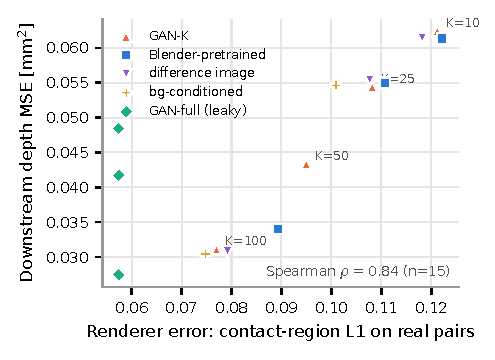
\includegraphics[width=0.9\columnwidth]{figures/fig_fidelity.pdf}
    \caption{\textbf{Renderer fidelity predicts downstream error.} Contact-region L1 between rendered and real images on held-out real (depth, image) pairs versus depth MSE of the downstream model trained with that renderer's synthetic data, for nine renderer variants. The relation is monotone; a renderer can be screened in minutes without downstream training.}
    \label{fig:fidelity}
\end{figure}

\noindent\textbf{A fidelity proxy.} Because every renderer maps depth to image, we can render the depth maps of the real validation pairs and compare with the real images directly. Fig.~\ref{fig:fidelity} plots the contact-region L1 of nine renderer variants against the downstream depth MSE obtained with their synthetic data: the ordering is preserved across families and budgets. The full-image L1 is dominated by the illumination field and is less predictive. This proxy costs seconds per renderer and we used it to screen the variants below before any downstream training.

\begin{table}[t]
\centering
\tableformat
\caption{\textbf{Appearance-side variants} at $\Kreal=25$ (real validation split) and leave-object-out (unseen objects). Renderer fidelity is the contact-region L1 of Fig.~\ref{fig:fidelity}. None of the variants improves contact depth without leakage.}
\label{tab:variants}
\begin{tabularx}{\columnwidth}{Xrrrr}
\toprule
& \multicolumn{2}{c}{$\Kreal=25$} & \multicolumn{2}{c}{Unseen objects} \\
\cmidrule(lr){2-3}\cmidrule(lr){4-5}
Variant & \shortstack[c]{\strut Fidelity\\\strut $\downarrow$} & \metrichead{Contact}{MAE} & \metrichead{Contact}{MAE} & \metrichead{Rot.}{(deg)} \\
\midrule
Real only & -- & 0.303 & 0.347 & 48.3 \\
Real only, bg-norm. & -- & 0.302 & 0.350 & 50.9 \\
GAN-$\Kreal$ / GAN-LOO & 0.108 & 0.318 & 0.333 & 7.6 \\
\quad Blender-pretrained & 0.111 & 0.335 & 0.356 & 8.5 \\
\quad difference-image & 0.108 & 0.339 & 0.346 & 6.3 \\
Blender & -- & 0.347 & 0.352 & 7.8 \\
Blender, bg-norm. & -- & 0.343 & 0.348 & 5.6 \\
\bottomrule
\end{tabularx}
\end{table}

\noindent\textbf{Which appearance factor limits few-shot fidelity?}
\label{sec:negative}
We tested three hypotheses (Table~\ref{tab:variants}).
\emph{(i) Missing physical prior.} A learned renderer with few pairs may lack the depth-to-shading structure that the physical renderer has for free. We pretrained the GAN on $30$k (depth, Blender image) pairs and fine-tuned it on the $\Kreal$ real pairs. Fidelity did not improve at any $\Kreal$ ($0.111$ vs.\ $0.108$ at $\Kreal=25$; $0.089$ vs.\ $0.077$ at $\Kreal=100$) and downstream depth was unchanged or worse.
\emph{(ii) Session illumination drift.} Because each object is one session, we measured the no-contact background of every session (per-pixel median over its frames). The backgrounds differ strongly: the mean blue channel ranges from $0.11$ to $0.38$ across sessions, and the between-session background difference ($0.05$--$0.10$ L1) exceeds the total error of the best renderer ($0.03$). A depth-conditioned renderer cannot know the session, so we normalized every frame (real and simulated) to a canonical background, $I \leftarrow I - B_{\mathrm{session}} + \bar B$, and trained a difference-image GAN that predicts $I-B_{\mathrm{session}}$. Full-image L1 improved by $13$--$21\%$, confirming the drift is real, but contact-region L1 did not move ($0.108$ at $\Kreal=25$) and contact MAE did not improve. The frozen sensor-invariant encoder is already robust to the illumination field; the only downstream effect of normalization is on pose transfer to unseen objects ($7.8^\circ\!\to\!5.6^\circ$ with the physical renderer), where a consistent background removes a spurious cue.
\emph{(iii) Contact shading.} What remains is the appearance \emph{inside} the contact region: the dark, low-contrast, gel-specific shading visible in the real column of Fig.~\ref{fig:renders}, which the physical renderer models with a hand-tuned darkening term and the learned renderer must learn from examples. Every result above is consistent with this being the limiting factor: strict renderers separate from real-only training only when they have seen enough contacts ($\Kreal\!\ge\!100$), leakage helps exactly because it exposes the test contacts, and the downstream errors are localization errors of the contact region (IoU $0.6$--$0.75$) rather than depth-magnitude errors (peak error $<0.1\,$mm).
